% Options for packages loaded elsewhere
\PassOptionsToPackage{unicode}{hyperref}
\PassOptionsToPackage{hyphens}{url}
%
\documentclass[
]{article}
\usepackage{lmodern}
\usepackage{amsmath}
\usepackage{ifxetex,ifluatex}
\ifnum 0\ifxetex 1\fi\ifluatex 1\fi=0 % if pdftex
  \usepackage[T1]{fontenc}
  \usepackage[utf8]{inputenc}
  \usepackage{textcomp} % provide euro and other symbols
  \usepackage{amssymb}
\else % if luatex or xetex
  \usepackage{unicode-math}
  \defaultfontfeatures{Scale=MatchLowercase}
  \defaultfontfeatures[\rmfamily]{Ligatures=TeX,Scale=1}
\fi
% Use upquote if available, for straight quotes in verbatim environments
\IfFileExists{upquote.sty}{\usepackage{upquote}}{}
\IfFileExists{microtype.sty}{% use microtype if available
  \usepackage[]{microtype}
  \UseMicrotypeSet[protrusion]{basicmath} % disable protrusion for tt fonts
}{}
\makeatletter
\@ifundefined{KOMAClassName}{% if non-KOMA class
  \IfFileExists{parskip.sty}{%
    \usepackage{parskip}
  }{% else
    \setlength{\parindent}{0pt}
    \setlength{\parskip}{6pt plus 2pt minus 1pt}}
}{% if KOMA class
  \KOMAoptions{parskip=half}}
\makeatother
\usepackage{xcolor}
\IfFileExists{xurl.sty}{\usepackage{xurl}}{} % add URL line breaks if available
\IfFileExists{bookmark.sty}{\usepackage{bookmark}}{\usepackage{hyperref}}
\hypersetup{
  pdftitle={Group\_01\_Project2\_demo},
  pdfauthor={Group\_01},
  hidelinks,
  pdfcreator={LaTeX via pandoc}}
\urlstyle{same} % disable monospaced font for URLs
\usepackage[margin=1in]{geometry}
\usepackage{longtable,booktabs}
\usepackage{calc} % for calculating minipage widths
% Correct order of tables after \paragraph or \subparagraph
\usepackage{etoolbox}
\makeatletter
\patchcmd\longtable{\par}{\if@noskipsec\mbox{}\fi\par}{}{}
\makeatother
% Allow footnotes in longtable head/foot
\IfFileExists{footnotehyper.sty}{\usepackage{footnotehyper}}{\usepackage{footnote}}
\makesavenoteenv{longtable}
\usepackage{graphicx}
\makeatletter
\def\maxwidth{\ifdim\Gin@nat@width>\linewidth\linewidth\else\Gin@nat@width\fi}
\def\maxheight{\ifdim\Gin@nat@height>\textheight\textheight\else\Gin@nat@height\fi}
\makeatother
% Scale images if necessary, so that they will not overflow the page
% margins by default, and it is still possible to overwrite the defaults
% using explicit options in \includegraphics[width, height, ...]{}
\setkeys{Gin}{width=\maxwidth,height=\maxheight,keepaspectratio}
% Set default figure placement to htbp
\makeatletter
\def\fps@figure{htbp}
\makeatother
\setlength{\emergencystretch}{3em} % prevent overfull lines
\providecommand{\tightlist}{%
  \setlength{\itemsep}{0pt}\setlength{\parskip}{0pt}}
\setcounter{secnumdepth}{-\maxdimen} % remove section numbering
\usepackage{booktabs}
\usepackage{longtable}
\usepackage{array}
\usepackage{multirow}
\usepackage{wrapfig}
\usepackage{float}
\usepackage{colortbl}
\usepackage{pdflscape}
\usepackage{tabu}
\usepackage{threeparttable}
\usepackage{threeparttablex}
\usepackage[normalem]{ulem}
\usepackage{makecell}
\usepackage{xcolor}
\ifluatex
  \usepackage{selnolig}  % disable illegal ligatures
\fi

\title{Group\_01\_Project2\_demo}
\author{Group\_01}
\date{}

\begin{document}
\maketitle

\hypertarget{sec:Intro}{%
\section{Introduction}\label{sec:Intro}}

Data come from the FIES (Family Income and Expenditure Survey) recorded
in the Philippines. The survey, which is undertaken every three years,
is aimed at providing data on family income and expenditure. The data
obtained from this survey are from different regions across the
Philippines. This report will focus on one individual area, the
Cordillera Administrative Region and so region has been removed from the
dataset as it will not be informative as an explanatory variable.

The report will investigate which household related variables influence
the number of people living in a household. The data used consists of
1725 observations of ten variables, two of which are categorical and the
remaining are numerical.

\hypertarget{sec:EDA}{%
\section{Exploratory Data Analysis}\label{sec:EDA}}

Figure 1 shows the distribution of the response variable: Number of
members in a household (variable name
``Total.number.of.family.members''). The modal response is 4 members and
the distribution is right-skewed,

\begin{figure}[H]

{\centering 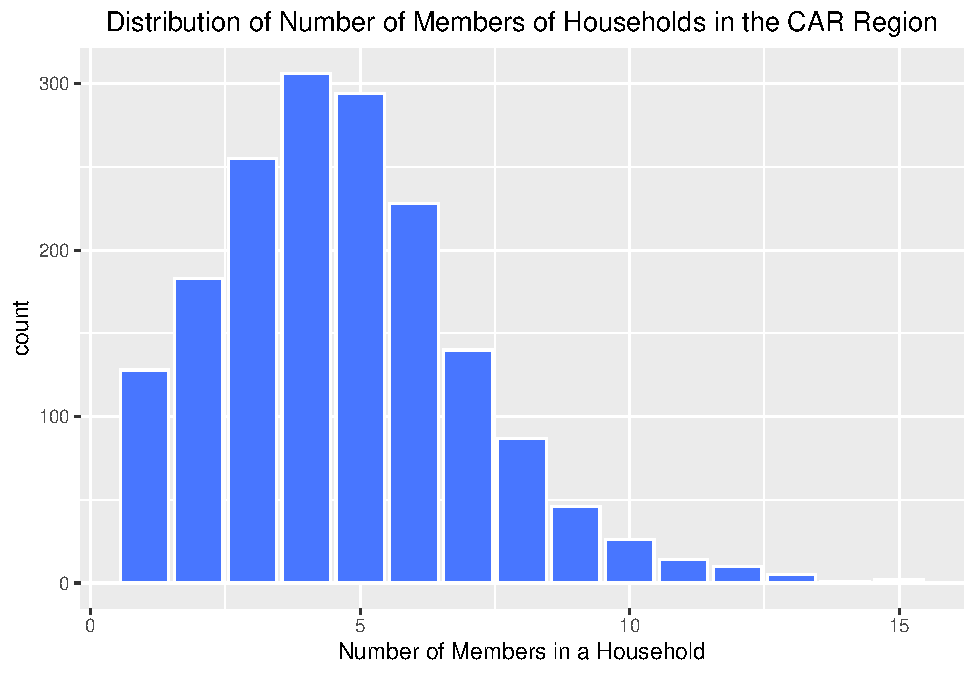
\includegraphics[width=0.8\linewidth]{Group_01_Project2_demo_files/figure-latex/distribution of response variable-1} 

}

\caption{Distribution of Response Variable}\label{fig:distribution of response variable}
\end{figure}

The summary below shows the count data for each level of the response
variable and the percentage of total households in the region in each
group.

\begin{verbatim}
 Total.Number.of.Family.members    n percent
                              1  128    7.4%
                              2  183   10.6%
                              3  255   14.8%
                              4  306   17.7%
                              5  294   17.0%
                              6  228   13.2%
                              7  140    8.1%
                              8   87    5.0%
                              9   46    2.7%
                             10   26    1.5%
                             11   14    0.8%
                             12   10    0.6%
                             13    5    0.3%
                             14    1    0.1%
                             15    2    0.1%
                          Total 1725  100.0%
\end{verbatim}

Figure 2 shows a graphical visualisation for all the variables in the
data set.

\begin{figure}[H]

{\centering 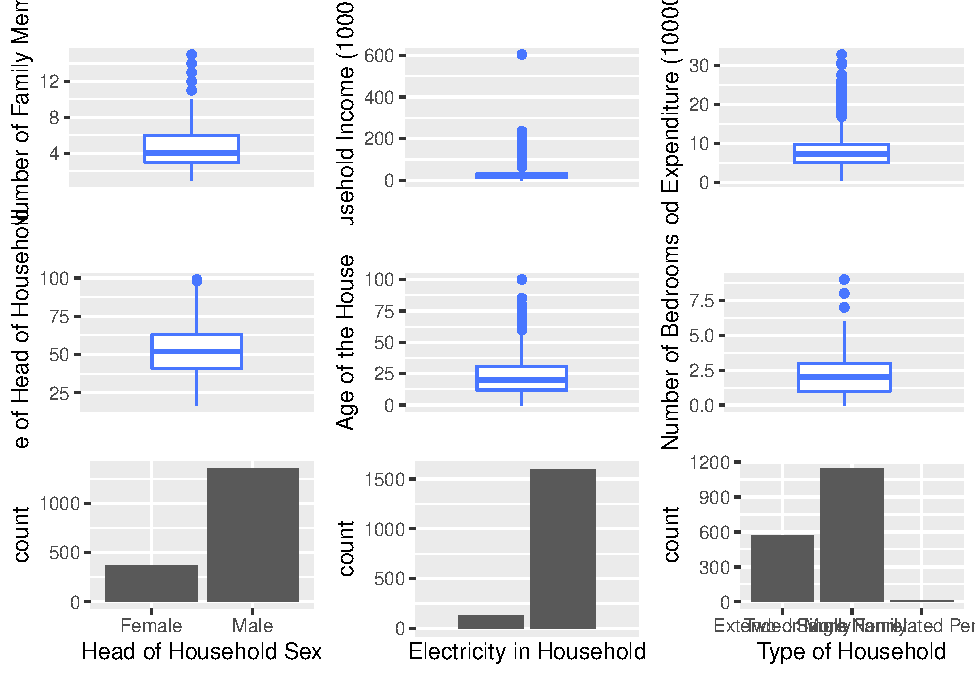
\includegraphics[width=0.8\linewidth]{Group_01_Project2_demo_files/figure-latex/all summaries-1} 

}

\caption{Graphical Summaries of Variables}\label{fig:all summaries}
\end{figure}

Table 1 shows summary data for all the numerical variables.There is no
missing data within these variables and so no values will need to be
imputed for the analysis in the report. The response variable, total
number of family members in a household, ranges from 1 to 15, with the
middle 50\% of number of family members falling between 3 and 6 also an
average number of family members of 4.67. There appear to be possible
outliers at the maximum values of Total Household Income and House Floor
Area. The total household income is range from 11988 to 6042860
Philippine Peso. The middle 50\% of total household income is between
118565 and 328335, with an income of 269540.48 peso on average. The
third variable is total food expenditure, in Phillipine peso, which is
the range of 6781 to 327724, with the middle 50\% lies between 51922 and
98493. Then, the household head's age is range from 17 to 99 years, with
the middle 50\% falling between 41 and 63 years of age. Next, the house
floor area is range from 5 to 900 square metres. The central 50\% of the
variable house floor area is between 32 and 102 with an average area of
90.92. The sixth explanatory variable is the house (building) age and it
ranges in value from 0 to 100, with the middle 50\% falling between 12
and 31. The number of bedrooms in the house ranges from 0 to 9 with a
mean average number of bedrooms of 2.26 per household. Finally, we may
look at the binary variable electricity, which denotes whether the
property has electricity access or not, the average score of electricity
is 0.93, which means 93\% household have electricity.

\begin{table}

\caption{\label{tab:numerical summaries}Summary statistics of numerical variables}
\centering
\resizebox{\linewidth}{!}{
\fontsize{10}{12}\selectfont
\begin{tabular}[t]{lrrrrrrrrr}
\toprule
Variable & Missing & Complete & Mean & SD & Min. & 1st Q. & Median & 3rd Q. & Max.\\
\midrule
Total.Number.of.Family.members & 0 & 1 & 4.67 & 2.33 & 1.00 & 3.00 & 4.00 & 6.00 & 15.00\\
Total.Household.Income & 0 & 1 & 26.95 & 27.46 & 1.20 & 11.86 & 18.86 & 32.83 & 604.29\\
Total.Food.Expenditure & 0 & 1 & 8.04 & 4.12 & 0.68 & 5.19 & 7.36 & 9.85 & 32.77\\
Household.Head.Age & 0 & 1 & 52.23 & 14.52 & 17.00 & 41.00 & 52.00 & 63.00 & 99.00\\
House.Floor.Area & 0 & 1 & 90.92 & 99.20 & 5.00 & 32.00 & 54.00 & 102.00 & 900.00\\
\addlinespace
House.Age & 0 & 1 & 22.98 & 15.32 & 0.00 & 12.00 & 20.00 & 31.00 & 100.00\\
Number.of.bedrooms & 0 & 1 & 2.26 & 1.44 & 0.00 & 1.00 & 2.00 & 3.00 & 9.00\\
Electricity & 0 & 1 & 0.93 & 0.26 & 0.00 & 1.00 & 1.00 & 1.00 & 1.00\\
\bottomrule
\end{tabular}}
\end{table}

The correlation coefficient between all numerical variables are shown in
Table 2. There is a moderate positive correlation (0.611) between the
total household income and the household food expenditure. Additionally
there is a slight positive correlation between the total household
income and the number of bedrooms in the household (0.441) and the
number of family members and total food expenditure (0.469). The other
variables are all weakly correlated.The correlation coefficient between
household Head's age, house floor area, house age and total number of
family members are negative, which shows the rise of those three
variables will lead to a reduction in the expected number of family
members in a household.

\begin{table}

\caption{\label{tab:correlation}Correlation of all variables.}
\centering
\resizebox{\linewidth}{!}{
\fontsize{10}{12}\selectfont
\begin{tabular}[t]{lrrrrrrrr}
\toprule
  & Total.Number.of.Family.members & Total.Household.Income & Total.Food.Expenditure & Household.Head.Age & House.Floor.Area & House.Age & Number.of.bedrooms & Electricity\\
\midrule
Total.Number.of.Family.members & 1.000 & 0.192 & 0.469 & -0.065 & -0.014 & -0.070 & 0.072 & 0.092\\
Total.Household.Income & 0.192 & 1.000 & 0.611 & 0.063 & 0.234 & 0.025 & 0.441 & 0.149\\
Total.Food.Expenditure & 0.469 & 0.611 & 1.000 & -0.052 & 0.124 & 0.007 & 0.356 & 0.199\\
Household.Head.Age & -0.065 & 0.063 & -0.052 & 1.000 & 0.091 & 0.218 & 0.154 & -0.013\\
House.Floor.Area & -0.014 & 0.234 & 0.124 & 0.091 & 1.000 & 0.074 & 0.374 & 0.107\\
\addlinespace
House.Age & -0.070 & 0.025 & 0.007 & 0.218 & 0.074 & 1.000 & 0.123 & 0.085\\
Number.of.bedrooms & 0.072 & 0.441 & 0.356 & 0.154 & 0.374 & 0.123 & 1.000 & 0.214\\
Electricity & 0.092 & 0.149 & 0.199 & -0.013 & 0.107 & 0.085 & 0.214 & 1.000\\
\bottomrule
\end{tabular}}
\end{table}

Table 3 shows the summaries of the two categorical variables. Single
family households make up approximately two-thirds of the survey
responses in this region and only 0.5\% (8) of responses came from
households formed from non-related individuals. Of the 1725 households,
less than a quarter (21.4\%) had a female head of household.

\begin{table}
\caption{\label{tab:categorical summaries}Summary of Categorial Explanatory Variables}

\centering
\begin{tabular}[middle]{lrl}
\toprule
Household.Head.Sex & n & percent\\
\midrule
Female & 369 & 21.4\%\\
Male & 1356 & 78.6\%\\
Total & 1725 & 100.0\%\\
\bottomrule
\end{tabular}
\centering
\begin{tabular}[middle]{lrl}
\toprule
Type.of.Household & n & percent\\
\midrule
Extended Family & 569 & 33.0\%\\
Single Family & 1148 & 66.6\%\\
Two or More Nonrelated Persons/Members & 8 & 0.5\%\\
Total & 1725 & 100.0\%\\
\bottomrule
\end{tabular}
\end{table}

The pairs plot in Figure 3 is colour coded to illustrate any differences
between the distributions of the quantitative variables when the head of
household sex is included as a factor. The plots suggest the sex of the
head of household may impact the number of family members in the
household and the age of the head of the household.

\begin{figure}[H]

{\centering 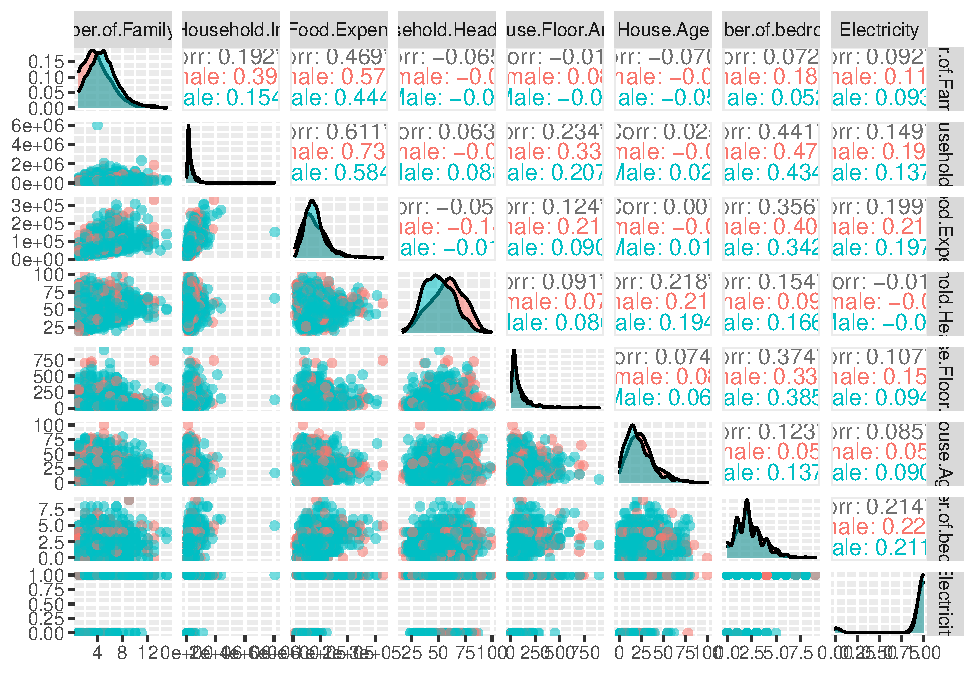
\includegraphics[width=1\linewidth]{Group_01_Project2_demo_files/figure-latex/pairs-1} 

}

\caption{Pair plots and correlation between numerical variables, colour coded to show the sex of the head of household.}\label{fig:pairs}
\end{figure}

Figure 4 shows that an extended family household or one formed by
non-related individuals is more likely to have a female head, whereas a
larger proportion of single family households have male heads.

\begin{figure}[H]

{\centering 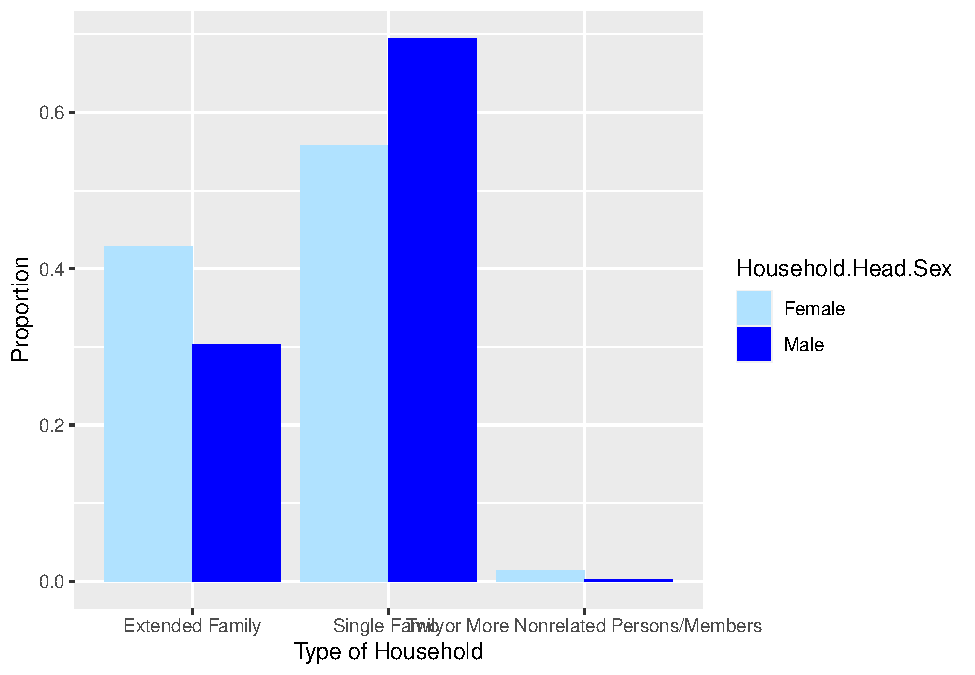
\includegraphics[width=0.8\linewidth]{Group_01_Project2_demo_files/figure-latex/barplot of sex by type of household-1} 

}

\caption{Barplot of household head's sex by type of household}\label{fig:barplot of sex by type of household}
\end{figure}

\begin{center}\rule{0.5\linewidth}{0.5pt}\end{center}

\newpage

\hypertarget{sec:ARC}{%
\section{Analysis of Relationships between Covariates}\label{sec:ARC}}

\hypertarget{gender-age}{%
\subsection{Gender \& Age}\label{gender-age}}

As highlighted by the pairs plot, there appears to be a relationship
between the sex and age of the head of the household.

The minimum and maximum ages of household heads do not appear to differ
greatly according to the individuals' sex, however they do differ at the
25th, 50th and 75th percentiles with male heads of households being
consitently younger than their female counterparts. The standard
deviation is also greater for the female group, but the substantially
smaller group size for females may contribute to this larger variation.

\begin{table}[!h]

\caption{\label{tab:summaries of age by sex}Summary statistics on the age of household heads by sex.}
\centering
\begin{tabular}[t]{l|r|r|r|r|r|r|r|r}
\hline
Household.Head.Sex & n & Mean & St.Dev & Min & Q1 & Median & Q3 & Max\\
\hline
Female & 369 & 58.23 & 15.69 & 17 & 47 & 59 & 69 & 99\\
\hline
Male & 1356 & 50.59 & 13.74 & 20 & 40 & 49 & 61 & 98\\
\hline
\end{tabular}
\end{table}

The boxplot in Figure 5 illustrates the previously summarised data. The
boxplot identifies the two oldest male head of households as outliers
(shown by the points above the whisker), however within the context of
the data and when compared to the ages of female head of household
boxplot, these ages do not appear unreasonable or unrealistic.

\begin{figure}

{\centering 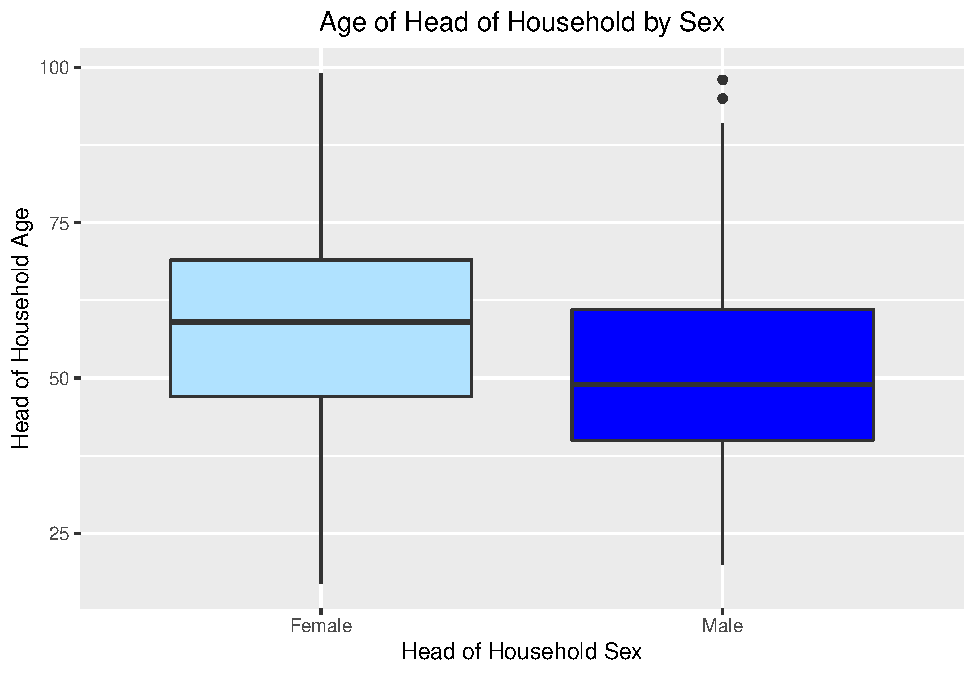
\includegraphics[width=0.8\linewidth]{Group_01_Project2_demo_files/figure-latex/boxplot of age by gender-1} 

}

\caption{Boxplots of Head of Household Age stratified by Sex}\label{fig:boxplot of age by gender}
\end{figure}

The following Mann-Whitney U-test shows that there is a statistically
significant difference in the median ages of male and female head of
households at a 5\% level.

\begin{verbatim}
    Wilcoxon rank sum test with continuity correction

data:  data.gender$Household.Head.Age by data.gender$Household.Head.Sex
W = 324284, p-value < 2.2e-16
alternative hypothesis: true location shift is not equal to 0
\end{verbatim}

\hypertarget{household-income-and-food-expenditure}{%
\subsection{Household Income and Food
Expenditure}\label{household-income-and-food-expenditure}}

Figure 6 shows a boxplot of household incomes suggests a heavily skewed
distribution with many outliers at the upper end of the distribution.

\begin{figure}[H]

{\centering 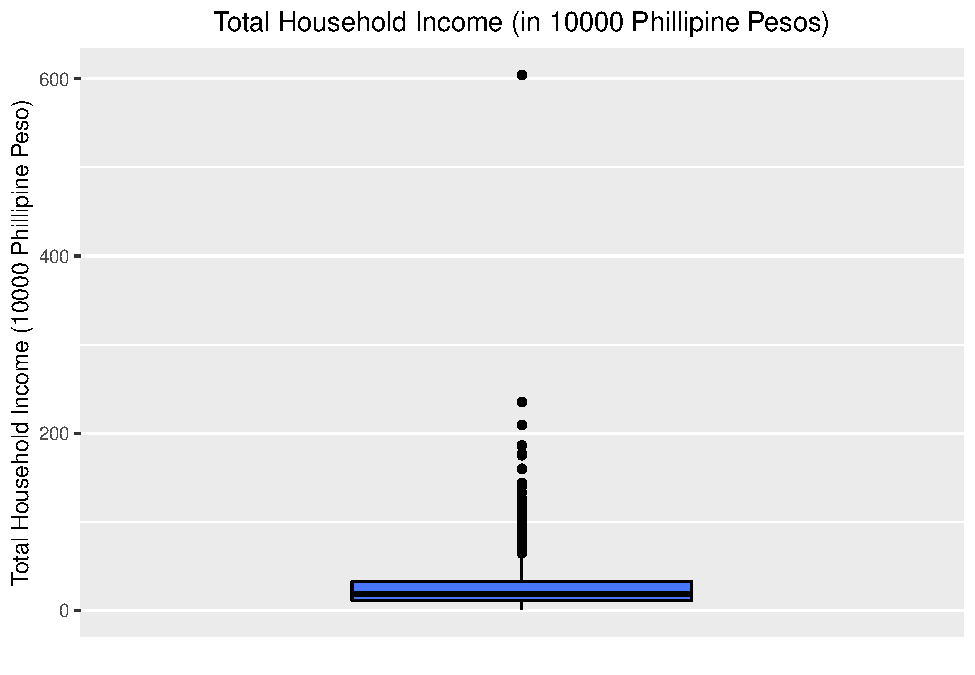
\includegraphics[width=0.8\linewidth]{Group_01_Project2_demo_files/figure-latex/balance boxplot-1} 

}

\caption{Household Incomes in 10000 Phillipine Pesos.}\label{fig:balance boxplot}
\end{figure}

The following boxplot in Figure 7 shows the log transformed household
income and shows there are still several outliers following the
transformation.

\begin{figure}[H]

{\centering 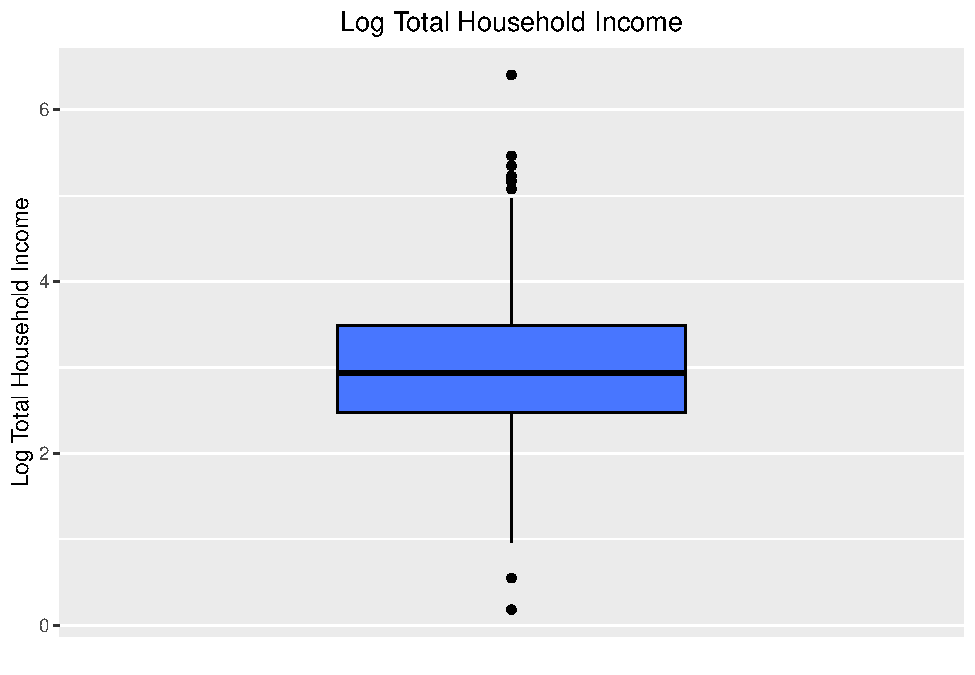
\includegraphics[width=0.8\linewidth]{Group_01_Project2_demo_files/figure-latex/balance boxplot2-1} 

}

\caption{Boxplot of log transformed Incomes.}\label{fig:balance boxplot2}
\end{figure}

The scatterplot in Figure 8 of household income against total food
expenditure suggests a positive correlation but the fitted model may be
being heavily influenced by the extreme values, particularly by one
extreme point.

\begin{figure}[H]

{\centering 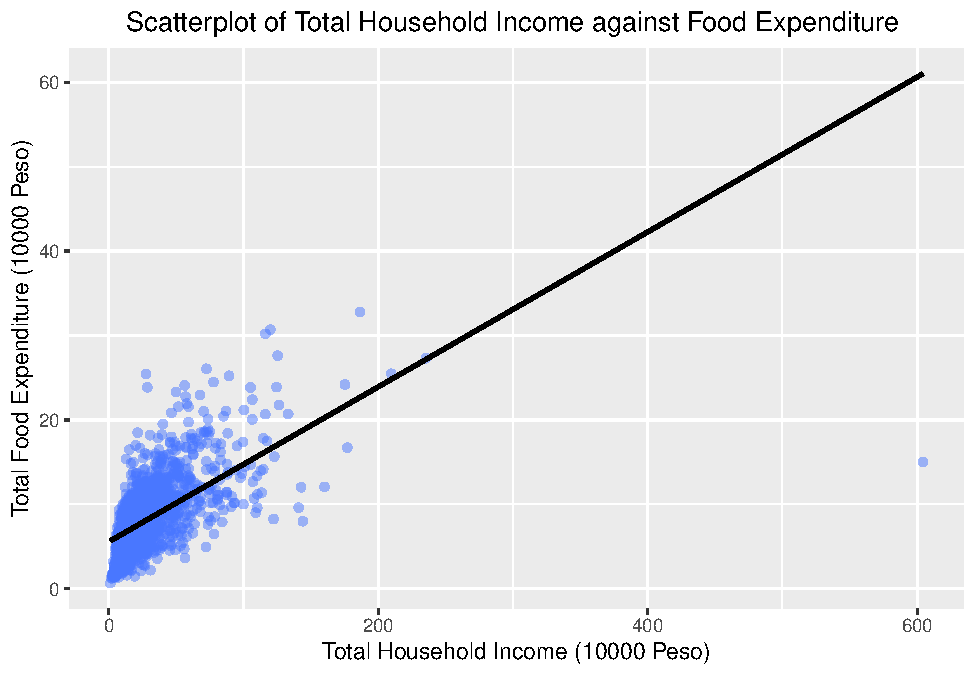
\includegraphics[width=0.8\linewidth]{Group_01_Project2_demo_files/figure-latex/balance_plot-1} 

}

\caption{Scatterplot of Income against Food Expenditure.}\label{fig:balance_plot}
\end{figure}

Figure 8 again highlights a possible outlier in terms of income, this
could be a data entry error or just an outlier at the maximum. Removing
this observation from the data set and plotting provides the following
scatter diagram in Figure 9. This plot reconfirms the suggested positive
correlation, but there is still an imbalance in the amount of data
available at different levels of income. For example, most data is
available for incomes between 0 and 750000 peso, but far fewer data
points occur above this income level.

\begin{figure}[H]

{\centering 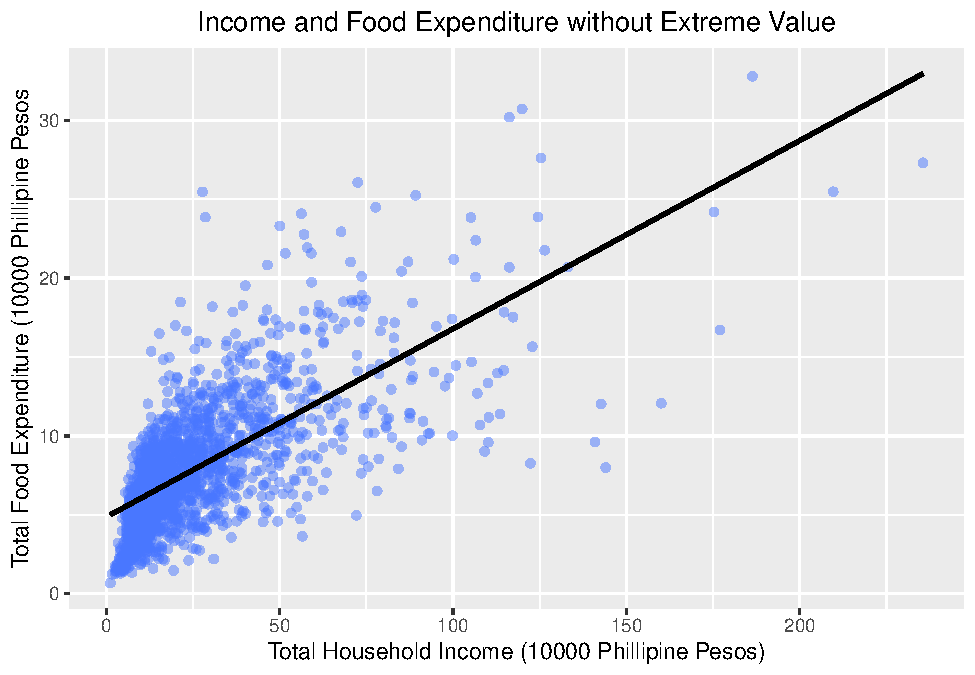
\includegraphics[width=0.8\linewidth]{Group_01_Project2_demo_files/figure-latex/balance without outlier-1} 

}

\caption{Scatterplot of Income and Food Expenditure with extreme value removed.}\label{fig:balance without outlier}
\end{figure}

\hypertarget{number-of-family-members-head-of-household-sex}{%
\subsection{Number of Family Members \& Head of Household
Sex}\label{number-of-family-members-head-of-household-sex}}

\begin{figure}[H]

{\centering 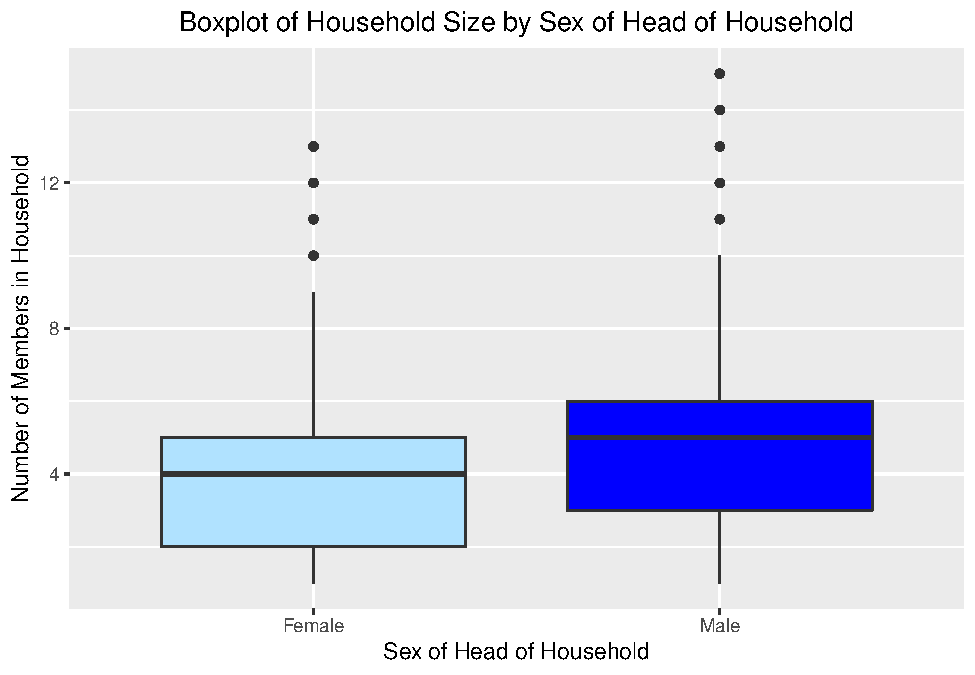
\includegraphics[width=0.8\linewidth]{Group_01_Project2_demo_files/figure-latex/boxplot of sex and members-1} 

}

\caption{Number of Members in Household by Sex of Head of Household}\label{fig:boxplot of sex and members}
\end{figure}

Hence we can see from Figure 10 that households with a male head appear
to have a greater number of family members on average than those with a
female head, as the male group has larger values for the first and third
quartiles and the median. However there is overlap between the two
groups central IQR and so the distributions may not be significantly
different.

\hypertarget{log-odds}{%
\paragraph{Log-odds}\label{log-odds}}

\begin{verbatim}
Call:
glm(formula = Household.Head.Sex ~ Total.Number.of.Family.members, 
    family = binomial(link = "logit"), data = data.sex_number)

Deviance Residuals: 
    Min       1Q   Median       3Q      Max  
-2.4219   0.4705   0.6602   0.7163   0.9054  

Coefficients:
                               Estimate Std. Error z value Pr(>|z|)    
(Intercept)                     0.49674    0.13174   3.771 0.000163 ***
Total.Number.of.Family.members  0.18319    0.02844   6.442 1.18e-10 ***
---
Signif. codes:  0 '***' 0.001 '**' 0.01 '*' 0.05 '.' 0.1 ' ' 1

(Dispersion parameter for binomial family taken to be 1)

    Null deviance: 1790.9  on 1724  degrees of freedom
Residual deviance: 1745.4  on 1723  degrees of freedom
AIC: 1749.4

Number of Fisher Scoring iterations: 4
\end{verbatim}

\begin{align} \ln\left(\frac{p}{1-p}\right) &= \alpha + \beta \cdot \textrm{number of family members} = 0.5 + 0.18 \cdot 
\textrm{number of family members}, \nonumber \end{align}

Where \(p = Prob(Male)\) and \(1-p = Prob(Female)\).

Hence, the log-odds of the household being male increase by 0.18 for
every one unit increase in number of family members. This provides us
with a point estimate of how the log-odds changes with age.

However, we are also interested in producing a 95\% confidence interval
for these log-odds.

\begin{longtable}[]{@{}lrr@{}}
\caption{95\% Confidence Interval for log-odds}\tabularnewline
\toprule
& 2.5 \% & 97.5 \%\tabularnewline
\midrule
\endfirsthead
\toprule
& 2.5 \% & 97.5 \%\tabularnewline
\midrule
\endhead
(Intercept) & 0.2388990 & 0.7555347\tabularnewline
Total.Number.of.Family.members & 0.1282353 & 0.2397474\tabularnewline
\bottomrule
\end{longtable}

\begin{figure}[H]

{\centering 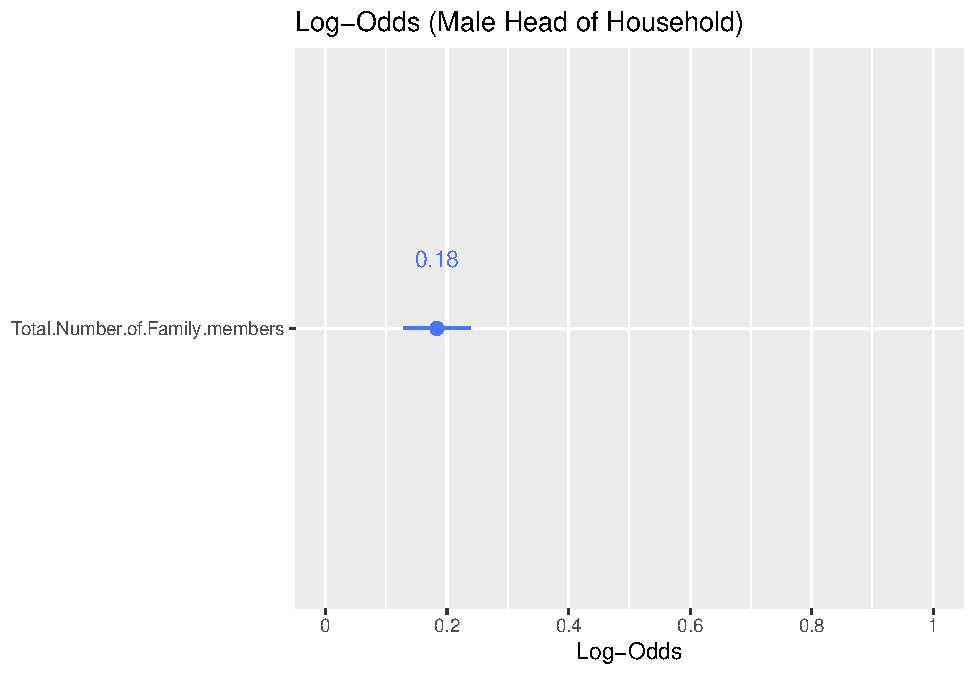
\includegraphics[width=0.8\linewidth]{Group_01_Project2_demo_files/figure-latex/plot of model-1} 

}

\caption{Log odds of a Male Head of Household}\label{fig:plot of model}
\end{figure}

Now, let's add the estimates of the log-odds to our data set:

\hypertarget{odds}{%
\paragraph{Odds}\label{odds}}

\begin{figure}[H]

{\centering 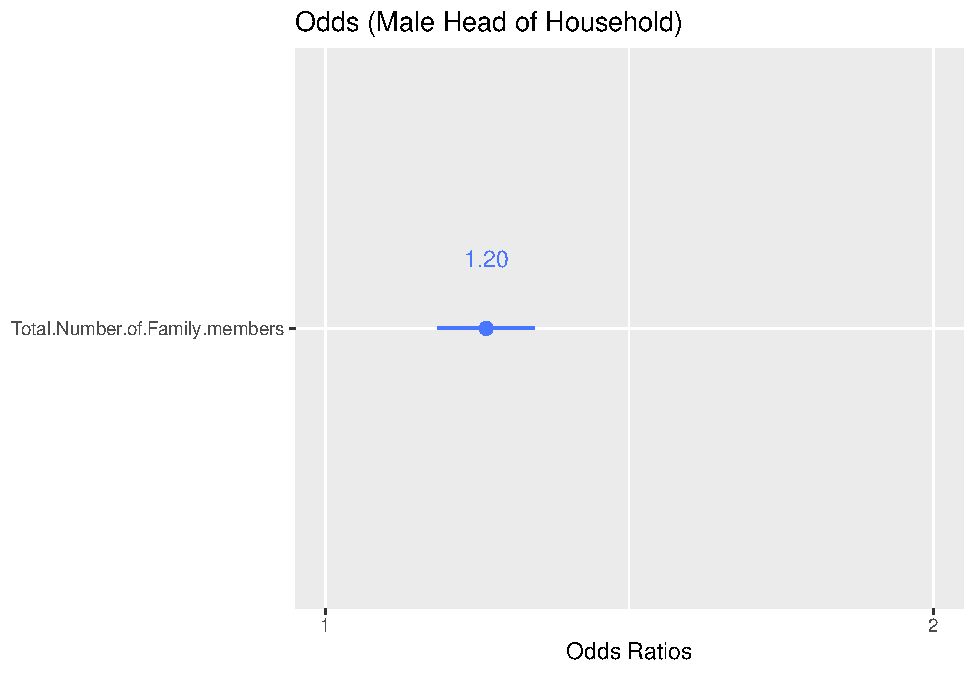
\includegraphics[width=0.8\linewidth]{Group_01_Project2_demo_files/figure-latex/model plot-1} 

}

\caption{Odds of a Male Head of Household}\label{fig:model plot}
\end{figure}

Now, let's add the estimates of the odds to our data set:

\hypertarget{probabilities}{%
\paragraph{Probabilities}\label{probabilities}}

\begin{figure}[H]

{\centering 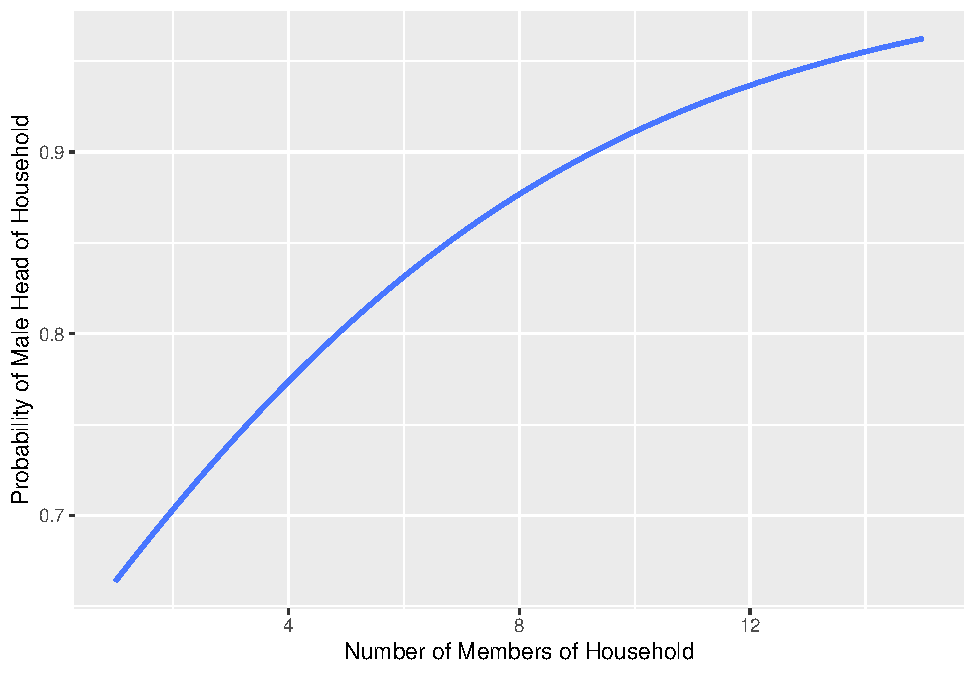
\includegraphics[width=0.8\linewidth]{Group_01_Project2_demo_files/figure-latex/probability plot-1} 

}

\caption{Probability of Male Head of Household given Number of Household Members}\label{fig:probability plot}
\end{figure}

\begin{verbatim}
$Total.Number.of.Family.members
\end{verbatim}

\begin{figure}[H]

{\centering 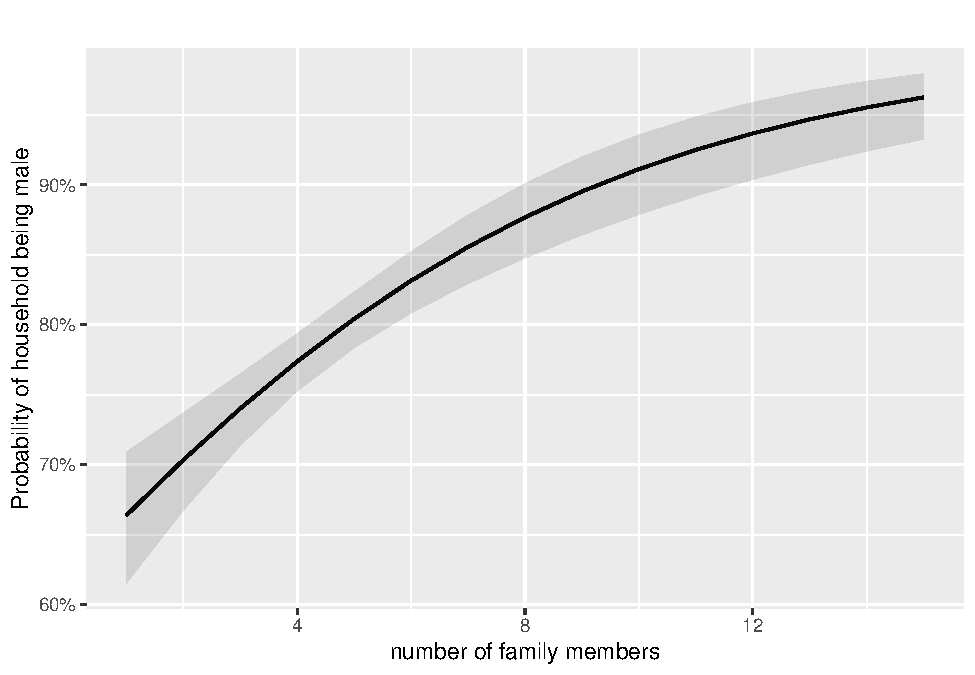
\includegraphics[width=0.8\linewidth]{Group_01_Project2_demo_files/figure-latex/probability plot 2-1} 

}

\caption{Predicted probability of Male Head of Households given Number of Household Members}\label{fig:probability plot 2}
\end{figure}

\begin{center}\rule{0.5\linewidth}{0.5pt}\end{center}

\newpage

\hypertarget{sec:EMA}{%
\section{Exploratory Model Analysis}\label{sec:EMA}}

\hypertarget{glm-model-exploration}{%
\subsection{GLM Model Exploration}\label{glm-model-exploration}}

Prior to exploring any models, the outlier for Total Household Income
and corresponding measurements for the other variables from this
individual are removed.

The following code identifies which explanatory variables would be
included to produce the best models of different sizes, in this instance
the maximum number of variables specified is ten. The output suggests
the first predictor to be included is the total food expenditure in
10000 Phillipine pesos, and the last to be included is the binary
variable Electricity that identifies if a household has electricity.
Comparing each of the ten models produced by BIC, CP and adjusted R\^{}2
criteria is inconclusive as each implies a different model is best.

\begin{verbatim}
Subset selection object
Call: regsubsets.formula(Total.Number.of.Family.members ~ ., data = data, 
    nvmax = 10)
10 Variables  (and intercept)
                                                        Forced in Forced out
Total.Household.Income                                      FALSE      FALSE
Total.Food.Expenditure                                      FALSE      FALSE
Household.Head.SexMale                                      FALSE      FALSE
Household.Head.Age                                          FALSE      FALSE
Type.of.HouseholdSingle Family                              FALSE      FALSE
Type.of.HouseholdTwo or More Nonrelated Persons/Members     FALSE      FALSE
House.Floor.Area                                            FALSE      FALSE
House.Age                                                   FALSE      FALSE
Number.of.bedrooms                                          FALSE      FALSE
Electricity                                                 FALSE      FALSE
1 subsets of each size up to 10
Selection Algorithm: exhaustive
          Total.Household.Income Total.Food.Expenditure Household.Head.SexMale
1  ( 1 )  " "                    "*"                    " "                   
2  ( 1 )  " "                    "*"                    " "                   
3  ( 1 )  " "                    "*"                    "*"                   
4  ( 1 )  "*"                    "*"                    "*"                   
5  ( 1 )  "*"                    "*"                    "*"                   
6  ( 1 )  "*"                    "*"                    "*"                   
7  ( 1 )  "*"                    "*"                    "*"                   
8  ( 1 )  "*"                    "*"                    "*"                   
9  ( 1 )  "*"                    "*"                    "*"                   
10  ( 1 ) "*"                    "*"                    "*"                   
          Household.Head.Age Type.of.HouseholdSingle Family
1  ( 1 )  " "                " "                           
2  ( 1 )  " "                "*"                           
3  ( 1 )  " "                "*"                           
4  ( 1 )  " "                "*"                           
5  ( 1 )  " "                "*"                           
6  ( 1 )  " "                "*"                           
7  ( 1 )  "*"                "*"                           
8  ( 1 )  "*"                "*"                           
9  ( 1 )  "*"                "*"                           
10  ( 1 ) "*"                "*"                           
          Type.of.HouseholdTwo or More Nonrelated Persons/Members
1  ( 1 )  " "                                                    
2  ( 1 )  " "                                                    
3  ( 1 )  " "                                                    
4  ( 1 )  " "                                                    
5  ( 1 )  " "                                                    
6  ( 1 )  " "                                                    
7  ( 1 )  " "                                                    
8  ( 1 )  " "                                                    
9  ( 1 )  "*"                                                    
10  ( 1 ) "*"                                                    
          House.Floor.Area House.Age Number.of.bedrooms Electricity
1  ( 1 )  " "              " "       " "                " "        
2  ( 1 )  " "              " "       " "                " "        
3  ( 1 )  " "              " "       " "                " "        
4  ( 1 )  " "              " "       " "                " "        
5  ( 1 )  " "              "*"       " "                " "        
6  ( 1 )  " "              "*"       "*"                " "        
7  ( 1 )  " "              "*"       "*"                " "        
8  ( 1 )  "*"              "*"       "*"                " "        
9  ( 1 )  "*"              "*"       "*"                " "        
10  ( 1 ) "*"              "*"       "*"                "*"        
\end{verbatim}

\begin{verbatim}
Adj.R2     CP    BIC 
     9      8      6 
\end{verbatim}

\hypertarget{gaussian-model}{%
\subsubsection{Gaussian Model}\label{gaussian-model}}

The following model includes each of the seven numerical explanatory
variables.

\begin{verbatim}
Call:
glm(formula = Total.Number.of.Family.members ~ Total.Household.Income + 
    Total.Food.Expenditure + Household.Head.Age + House.Floor.Area + 
    House.Age + Number.of.bedrooms + Electricity, data = data)

Deviance Residuals: 
    Min       1Q   Median       3Q      Max  
-5.7591  -1.4530  -0.2764   1.1867  10.7642  

Coefficients:
                         Estimate Std. Error t value Pr(>|t|)    
(Intercept)             2.6971922  0.2674785  10.084  < 2e-16 ***
Total.Household.Income -0.0142415  0.0030770  -4.628 3.96e-06 ***
Total.Food.Expenditure  0.3328803  0.0166592  19.982  < 2e-16 ***
Household.Head.Age     -0.0002507  0.0035178  -0.071  0.94320    
House.Floor.Area       -0.0006203  0.0005377  -1.154  0.24882    
House.Age              -0.0094813  0.0032978  -2.875  0.00409 ** 
Number.of.bedrooms     -0.0842340  0.0416746  -2.021  0.04341 *  
Electricity             0.1679324  0.1927530   0.871  0.38375    
---
Signif. codes:  0 '***' 0.001 '**' 0.01 '*' 0.05 '.' 0.1 ' ' 1

(Dispersion parameter for gaussian family taken to be 4.123137)

    Null deviance: 9383.5  on 1723  degrees of freedom
Residual deviance: 7075.3  on 1716  degrees of freedom
AIC: 7344.7

Number of Fisher Scoring iterations: 2
\end{verbatim}

The fitted model identifies four significant (at the 5\% level)
explanatory variables which are: - Total Household Income - Total Food
Expenditure - Age of the Building - Number of Bedrooms

Refitting the model to include the previously identified significant
predictors.

\begin{verbatim}
Call:
glm(formula = Total.Number.of.Family.members ~ Total.Household.Income + 
    Total.Food.Expenditure + House.Age + Number.of.bedrooms, 
    data = data)

Deviance Residuals: 
    Min       1Q   Median       3Q      Max  
-5.7811  -1.4397  -0.2775   1.1774  10.6633  

Coefficients:
                        Estimate Std. Error t value Pr(>|t|)    
(Intercept)             2.788740   0.138543  20.129  < 2e-16 ***
Total.Household.Income -0.014790   0.003037  -4.870 1.22e-06 ***
Total.Food.Expenditure  0.336500   0.016337  20.597  < 2e-16 ***
House.Age              -0.009457   0.003219  -2.938  0.00335 ** 
Number.of.bedrooms     -0.093392   0.039276  -2.378  0.01752 *  
---
Signif. codes:  0 '***' 0.001 '**' 0.01 '*' 0.05 '.' 0.1 ' ' 1

(Dispersion parameter for gaussian family taken to be 4.120847)

    Null deviance: 9383.5  on 1723  degrees of freedom
Residual deviance: 7083.7  on 1719  degrees of freedom
AIC: 7340.8

Number of Fisher Scoring iterations: 2
\end{verbatim}

Comparing the model with all numerical predictors and the model with the
identified significant predictors using the AIC and BIC model selection
criteria suggests the model with only the significant predictors is a
better fit for the data. Additionally, the latter model results in a
decrease of 2299.8 in the deviance with a loss of 4 degrees of freedom,
whereas the full numerical model had a reduction in deviance of 2308.2
with a loss of 7 degrees of freedom.

\begin{table}[H]

\caption{\label{tab:model comparison}Comparison of Fitted Models by AIC and BIC criteria }
\centering
\begin{tabular}[t]{lrr}
\toprule
Model & AIC & BIC\\
\midrule
Full Numerical Model & 7344.72 & 7393.80\\
Significant Predictors Model & 7340.78 & 7373.49\\
\bottomrule
\end{tabular}
\end{table}

\hypertarget{binomial-model}{%
\subsubsection{Binomial Model}\label{binomial-model}}

The following code assigns the response variable and categorical
explanatory variables as factors. Treating each different number of
household members as a different level of the response variable allows a
binomial model to be fitted with the logit link function.

The model is fitted to include all explanatory variables, categorical
and numerical. This model identifies three statistically significant
explanatory variables: Total Household Income (in ten thousand
Philippine Pesos), Total Food Expenditure (in ten thousand Phillipine
Pesos) and the Head of Household Sex being male (female is treated as
the baseline). For an increase of 10000 peso in the total household
income, the number of household members decreases by 0.03557. An
increase of 10000 peso in Food Expenditure results in an increase of
1.048 in the number of household members. If the Head of Household is
Male it is expected there will be 1.143 more household members than if
the Head of the Household is Female.

\begin{verbatim}
Call:
glm(formula = Total.Number.of.Family.members ~ Total.Household.Income + 
    Total.Food.Expenditure + Household.Head.Sex + Household.Head.Age + 
    Type.of.Household + House.Floor.Area + House.Age + Number.of.bedrooms + 
    Electricity, family = binomial(link = "logit"), data = data)

Deviance Residuals: 
    Min       1Q   Median       3Q      Max  
-4.2298   0.0000   0.0293   0.1948   1.8561  

Coefficients:
                                                          Estimate Std. Error
(Intercept)                                              1.438e+01  5.696e+02
Total.Household.Income                                  -3.557e-02  1.017e-02
Total.Food.Expenditure                                   1.048e+00  9.895e-02
Household.Head.SexMale                                   1.143e+00  2.734e-01
Household.Head.Age                                      -5.534e-03  7.499e-03
Type.of.HouseholdSingle Family                          -1.737e+01  5.696e+02
Type.of.HouseholdTwo or More Nonrelated Persons/Members -2.952e+00  5.612e+03
House.Floor.Area                                         1.484e-03  1.224e-03
House.Age                                               -9.422e-04  7.817e-03
Number.of.bedrooms                                      -1.774e-01  1.034e-01
Electricity                                              3.235e-01  3.411e-01
                                                        z value Pr(>|z|)    
(Intercept)                                               0.025 0.979863    
Total.Household.Income                                   -3.497 0.000471 ***
Total.Food.Expenditure                                   10.595  < 2e-16 ***
Household.Head.SexMale                                    4.181 2.91e-05 ***
Household.Head.Age                                       -0.738 0.460510    
Type.of.HouseholdSingle Family                           -0.030 0.975675    
Type.of.HouseholdTwo or More Nonrelated Persons/Members  -0.001 0.999580    
House.Floor.Area                                          1.212 0.225414    
House.Age                                                -0.121 0.904055    
Number.of.bedrooms                                       -1.715 0.086317 .  
Electricity                                               0.948 0.343015    
---
Signif. codes:  0 '***' 0.001 '**' 0.01 '*' 0.05 '.' 0.1 ' ' 1

(Dispersion parameter for binomial family taken to be 1)

    Null deviance: 911.95  on 1723  degrees of freedom
Residual deviance: 448.76  on 1713  degrees of freedom
AIC: 470.76

Number of Fisher Scoring iterations: 19
\end{verbatim}

As the exploratory analysis of the data suggests sex of the head of the
household may interact with other variables, the following model is
fitted to include these interactions. This model returns six significant
predictors at the 5\% level however the values of some of these
coefficients are relatively small in the context of the data. For an
increase of 10000 peso in food expenditure, there is an increase of
0.728 in the number of household members. If the head of the household
is male then there is a further expected increase of 0.518 in household
members for this same rise in food expenditure. A one year increase in
the age of the head of the household results in a decrease of 0.036 in
the number of household members. However if the head of the household is
male then there is an additional increase of 0.042 in the number of
household members for every one year older. The remaining significant
coefficients imply that a 1 square-metre increase in floor area
correlates to a 0.006 increase in household members and finally in a
male led household with electricity it is expected there will be an
additional 1.999 members of the household.

\begin{verbatim}
Call:
glm(formula = Total.Number.of.Family.members ~ (Total.Household.Income + 
    Total.Food.Expenditure + Household.Head.Age + Type.of.Household + 
    House.Floor.Area + House.Age + Number.of.bedrooms + Electricity) * 
    Household.Head.Sex, family = binomial(link = "logit"), data = data)

Deviance Residuals: 
    Min       1Q   Median       3Q      Max  
-3.8031   0.0000   0.0180   0.1654   1.8853  

Coefficients:
                                                                                 Estimate
(Intercept)                                                                     1.947e+01
Total.Household.Income                                                         -1.270e-02
Total.Food.Expenditure                                                          7.284e-01
Household.Head.Age                                                             -3.633e-02
Type.of.HouseholdSingle Family                                                 -1.863e+01
Type.of.HouseholdTwo or More Nonrelated Persons/Members                        -3.269e+00
House.Floor.Area                                                                6.403e-03
House.Age                                                                      -2.041e-03
Number.of.bedrooms                                                             -1.696e-01
Electricity                                                                    -1.269e+00
Household.Head.SexMale                                                         -6.859e+00
Total.Household.Income:Household.Head.SexMale                                  -2.883e-02
Total.Food.Expenditure:Household.Head.SexMale                                   5.175e-01
Household.Head.Age:Household.Head.SexMale                                       4.213e-02
Type.of.HouseholdSingle Family:Household.Head.SexMale                           2.764e+00
Type.of.HouseholdTwo or More Nonrelated Persons/Members:Household.Head.SexMale  1.382e+00
House.Floor.Area:Household.Head.SexMale                                        -6.356e-03
House.Age:Household.Head.SexMale                                                2.190e-03
Number.of.bedrooms:Household.Head.SexMale                                      -3.488e-02
Electricity:Household.Head.SexMale                                              1.999e+00
                                                                               Std. Error
(Intercept)                                                                     1.143e+03
Total.Household.Income                                                          2.334e-02
Total.Food.Expenditure                                                          1.502e-01
Household.Head.Age                                                              1.423e-02
Type.of.HouseholdSingle Family                                                  1.143e+03
Type.of.HouseholdTwo or More Nonrelated Persons/Members                         7.482e+03
House.Floor.Area                                                                3.016e-03
House.Age                                                                       1.535e-02
Number.of.bedrooms                                                              2.101e-01
Electricity                                                                     7.165e-01
Household.Head.SexMale                                                          1.325e+03
Total.Household.Income:Household.Head.SexMale                                   2.612e-02
Total.Food.Expenditure:Household.Head.SexMale                                   2.026e-01
Household.Head.Age:Household.Head.SexMale                                       1.702e-02
Type.of.HouseholdSingle Family:Household.Head.SexMale                           1.325e+03
Type.of.HouseholdTwo or More Nonrelated Persons/Members:Household.Head.SexMale  1.156e+04
House.Floor.Area:Household.Head.SexMale                                         3.348e-03
House.Age:Household.Head.SexMale                                                1.807e-02
Number.of.bedrooms:Household.Head.SexMale                                       2.451e-01
Electricity:Household.Head.SexMale                                              8.175e-01
                                                                               z value
(Intercept)                                                                      0.017
Total.Household.Income                                                          -0.544
Total.Food.Expenditure                                                           4.849
Household.Head.Age                                                              -2.552
Type.of.HouseholdSingle Family                                                  -0.016
Type.of.HouseholdTwo or More Nonrelated Persons/Members                          0.000
House.Floor.Area                                                                 2.123
House.Age                                                                       -0.133
Number.of.bedrooms                                                              -0.807
Electricity                                                                     -1.772
Household.Head.SexMale                                                          -0.005
Total.Household.Income:Household.Head.SexMale                                   -1.104
Total.Food.Expenditure:Household.Head.SexMale                                    2.554
Household.Head.Age:Household.Head.SexMale                                        2.476
Type.of.HouseholdSingle Family:Household.Head.SexMale                            0.002
Type.of.HouseholdTwo or More Nonrelated Persons/Members:Household.Head.SexMale   0.000
House.Floor.Area:Household.Head.SexMale                                         -1.899
House.Age:Household.Head.SexMale                                                 0.121
Number.of.bedrooms:Household.Head.SexMale                                       -0.142
Electricity:Household.Head.SexMale                                               2.445
                                                                               Pr(>|z|)
(Intercept)                                                                      0.9864
Total.Household.Income                                                           0.5863
Total.Food.Expenditure                                                         1.24e-06
Household.Head.Age                                                               0.0107
Type.of.HouseholdSingle Family                                                   0.9870
Type.of.HouseholdTwo or More Nonrelated Persons/Members                          0.9997
House.Floor.Area                                                                 0.0337
House.Age                                                                        0.8942
Number.of.bedrooms                                                               0.4197
Electricity                                                                      0.0765
Household.Head.SexMale                                                           0.9959
Total.Household.Income:Household.Head.SexMale                                    0.2698
Total.Food.Expenditure:Household.Head.SexMale                                    0.0107
Household.Head.Age:Household.Head.SexMale                                        0.0133
Type.of.HouseholdSingle Family:Household.Head.SexMale                            0.9983
Type.of.HouseholdTwo or More Nonrelated Persons/Members:Household.Head.SexMale   0.9999
House.Floor.Area:Household.Head.SexMale                                          0.0576
House.Age:Household.Head.SexMale                                                 0.9035
Number.of.bedrooms:Household.Head.SexMale                                        0.8868
Electricity:Household.Head.SexMale                                               0.0145
                                                                                  
(Intercept)                                                                       
Total.Household.Income                                                            
Total.Food.Expenditure                                                         ***
Household.Head.Age                                                             *  
Type.of.HouseholdSingle Family                                                    
Type.of.HouseholdTwo or More Nonrelated Persons/Members                           
House.Floor.Area                                                               *  
House.Age                                                                         
Number.of.bedrooms                                                                
Electricity                                                                    .  
Household.Head.SexMale                                                            
Total.Household.Income:Household.Head.SexMale                                     
Total.Food.Expenditure:Household.Head.SexMale                                  *  
Household.Head.Age:Household.Head.SexMale                                      *  
Type.of.HouseholdSingle Family:Household.Head.SexMale                             
Type.of.HouseholdTwo or More Nonrelated Persons/Members:Household.Head.SexMale    
House.Floor.Area:Household.Head.SexMale                                        .  
House.Age:Household.Head.SexMale                                                  
Number.of.bedrooms:Household.Head.SexMale                                         
Electricity:Household.Head.SexMale                                             *  
---
Signif. codes:  0 '***' 0.001 '**' 0.01 '*' 0.05 '.' 0.1 ' ' 1

(Dispersion parameter for binomial family taken to be 1)

    Null deviance: 911.95  on 1723  degrees of freedom
Residual deviance: 426.70  on 1704  degrees of freedom
AIC: 466.7

Number of Fisher Scoring iterations: 19
\end{verbatim}

\begin{table}[H]

\caption{\label{tab:binomial glm model comparison}Binomial GLM Model Comparison by AIC and BIC}
\centering
\begin{tabular}[t]{lrr}
\toprule
Model & AIC & BIC\\
\midrule
No Interactions & 470.76 & 530.73\\
Interactions with Head of Household Sex & 466.70 & 575.75\\
\bottomrule
\end{tabular}
\end{table}

\begin{center}\rule{0.5\linewidth}{0.5pt}\end{center}

\newpage

\hypertarget{sec:FMA}{%
\section{Formal Model Analysis}\label{sec:FMA}}

\hypertarget{poisson-regression-model}{%
\subsection{Poisson Regression model}\label{poisson-regression-model}}

The response variable of the Total Number of Family Members (or members
of the household) can be viewed as a count and therefore a Poisson
Regression model is considered. For a Poisson model to be suitable, the
mean and variance should be equal and so these assumptions are checked
first.

\begin{table}

\caption{\label{tab:poisson mean and variance check}Mean and Variation of Response Variable}
\centering
\begin{tabular}[t]{l|r}
\hline
  & \\
\hline
Mean & 4.669373\\
\hline
Variance & 5.446049\\
\hline
\end{tabular}
\end{table}

The variation of total number of family members is only marginally
larger than the mean of total number of family members, thus, the
possibility of over-dispersion in our model is not a significant issue.

\begin{verbatim}
Call:
glm(formula = Total.Number.of.Family.members ~ Total.Household.Income + 
    Total.Food.Expenditure + Household.Head.Age + House.Floor.Area + 
    House.Age + Number.of.bedrooms + Electricity + Household.Head.Sex + 
    Type.of.Household, family = poisson(link = "log"), data = data)

Deviance Residuals: 
    Min       1Q   Median       3Q      Max  
-2.7749  -0.6993  -0.1044   0.4989   3.7501  

Coefficients:
                                                          Estimate Std. Error
(Intercept)                                              1.4254422  0.0796515
Total.Household.Income                                  -0.0022045  0.0006612
Total.Food.Expenditure                                   0.0500316  0.0035528
Household.Head.Age                                      -0.0025205  0.0008707
House.Floor.Area                                        -0.0001932  0.0001281
House.Age                                               -0.0023168  0.0007735
Number.of.bedrooms                                      -0.0145830  0.0095600
Electricity                                              0.0276347  0.0475502
Household.Head.SexMale                                   0.2202770  0.0297157
Type.of.HouseholdSingle Family                          -0.3481835  0.0248020
Type.of.HouseholdTwo or More Nonrelated Persons/Members -0.1444455  0.1598841
                                                        z value Pr(>|z|)    
(Intercept)                                              17.896  < 2e-16 ***
Total.Household.Income                                   -3.334 0.000856 ***
Total.Food.Expenditure                                   14.082  < 2e-16 ***
Household.Head.Age                                       -2.895 0.003793 ** 
House.Floor.Area                                         -1.509 0.131385    
House.Age                                                -2.995 0.002744 ** 
Number.of.bedrooms                                       -1.525 0.127155    
Electricity                                               0.581 0.561126    
Household.Head.SexMale                                    7.413 1.24e-13 ***
Type.of.HouseholdSingle Family                          -14.039  < 2e-16 ***
Type.of.HouseholdTwo or More Nonrelated Persons/Members  -0.903 0.366293    
---
Signif. codes:  0 '***' 0.001 '**' 0.01 '*' 0.05 '.' 0.1 ' ' 1

(Dispersion parameter for poisson family taken to be 1)

    Null deviance: 2024.3  on 1723  degrees of freedom
Residual deviance: 1330.4  on 1713  degrees of freedom
AIC: 7011.6

Number of Fisher Scoring iterations: 4
\end{verbatim}

The poisson model fitted with all possible covariates concludes there
are six statistically significant predictors at the 5\% level. These are
the total household income and food expenditure, the age and gender of
the head of the household, the age of the house and if it is a single
family household. Table 5 shows the estimates and the lower and upper
bounds of the 95\% confidence intervals for the regression parameters.
The rows containing significant predictors, and so where the confidence
intervals do not include 0, are highlighted.

\textbackslash begin\{table\}

\textbackslash caption\{\label{tab:table of estimates and confidence intervals}Estimates
and the corresponding 95\% Confidence Intervals, with significant
predictors highlighted.\} \centering

\begin{tabular}[t]{l|r|r|r}
\hline
  & Lower Bound & Estimate & Upper Bound\\
\hline
\cellcolor[HTML]{A1E8F1}{\textcolor{black}{(Intercept)}} & \cellcolor[HTML]{A1E8F1}{\textcolor{black}{1.2687606}} & \cellcolor[HTML]{A1E8F1}{\textcolor{black}{1.4254422}} & \cellcolor[HTML]{A1E8F1}{\textcolor{black}{1.5810043}}\\
\hline
\cellcolor[HTML]{A1E8F1}{\textcolor{black}{Total.Household.Income}} & \cellcolor[HTML]{A1E8F1}{\textcolor{black}{-0.0035110}} & \cellcolor[HTML]{A1E8F1}{\textcolor{black}{-0.0022045}} & \cellcolor[HTML]{A1E8F1}{\textcolor{black}{-0.0009192}}\\
\hline
\cellcolor[HTML]{A1E8F1}{\textcolor{black}{Total.Food.Expenditure}} & \cellcolor[HTML]{A1E8F1}{\textcolor{black}{0.0430507}} & \cellcolor[HTML]{A1E8F1}{\textcolor{black}{0.0500316}} & \cellcolor[HTML]{A1E8F1}{\textcolor{black}{0.0569775}}\\
\hline
\cellcolor[HTML]{A1E8F1}{\textcolor{black}{Household.Head.Age}} & \cellcolor[HTML]{A1E8F1}{\textcolor{black}{-0.0042279}} & \cellcolor[HTML]{A1E8F1}{\textcolor{black}{-0.0025205}} & \cellcolor[HTML]{A1E8F1}{\textcolor{black}{-0.0008148}}\\
\hline
House.Floor.Area & -0.0004469 & -0.0001932 & 0.0000552\\
\hline
\cellcolor[HTML]{A1E8F1}{\textcolor{black}{House.Age}} & \cellcolor[HTML]{A1E8F1}{\textcolor{black}{-0.0038392}} & \cellcolor[HTML]{A1E8F1}{\textcolor{black}{-0.0023168}} & \cellcolor[HTML]{A1E8F1}{\textcolor{black}{-0.0008069}}\\
\hline
Number.of.bedrooms & -0.0333633 & -0.0145830 & 0.0041111\\
\hline
Electricity & -0.0644803 & 0.0276347 & 0.1219537\\
\hline
\cellcolor[HTML]{A1E8F1}{\textcolor{black}{Household.Head.SexMale}} & \cellcolor[HTML]{A1E8F1}{\textcolor{black}{0.1623556}} & \cellcolor[HTML]{A1E8F1}{\textcolor{black}{0.2202770}} & \cellcolor[HTML]{A1E8F1}{\textcolor{black}{0.2788479}}\\
\hline
\cellcolor[HTML]{A1E8F1}{\textcolor{black}{Type.of.HouseholdSingle Family}} & \cellcolor[HTML]{A1E8F1}{\textcolor{black}{-0.3967514}} & \cellcolor[HTML]{A1E8F1}{\textcolor{black}{-0.3481835}} & \cellcolor[HTML]{A1E8F1}{\textcolor{black}{-0.2995260}}\\
\hline
Type.of.HouseholdTwo or More Nonrelated Persons/Members & -0.4743426 & -0.1444455 & 0.1540719\\
\hline
\end{tabular}

\textbackslash end\{table\}

We refit the model to include just the previously identified significant
covariates and again evaluated the 95\% confidence intervals for the
estimated parameters, these values can be seen in Table 6. The intercept
term of 1.436 is simply a positional constant due to the context of the
variables. The negative coefficient of Total Household Income shows that
for every additional 10000 peso, the number of household members is
expected to decrease by 0.002. The coefficient of Total Food Expenditure
suggests that for an increase of 10000 peso in spending, there is an
expected 0.048 more members in the household. The coefficients of Head
of Household age and the Age of the Building are both negative (-0.003
and -0.002 respectively) showing that an older head of the household or
older building is linked to fewer members in a household. A Single
Family household is expected to have 0.350 fewer members than the
baseline category of an extended family household, and households with a
male head will have 0.222 members more than their female counterparts.

\begin{verbatim}
Call:
glm(formula = Total.Number.of.Family.members ~ Total.Household.Income + 
    Total.Food.Expenditure + Household.Head.Age + House.Age + 
    Household.Head.Sex + Type.of.Household, family = poisson(link = "log"), 
    data = data)

Deviance Residuals: 
    Min       1Q   Median       3Q      Max  
-2.7325  -0.7095  -0.1012   0.5090   3.7690  

Coefficients:
                                                          Estimate Std. Error
(Intercept)                                              1.4313832  0.0672809
Total.Household.Income                                  -0.0028211  0.0006146
Total.Food.Expenditure                                   0.0503772  0.0035264
Household.Head.Age                                      -0.0027721  0.0008627
House.Age                                               -0.0024807  0.0007682
Household.Head.SexMale                                   0.2205681  0.0297155
Type.of.HouseholdSingle Family                          -0.3484617  0.0247448
Type.of.HouseholdTwo or More Nonrelated Persons/Members -0.1365104  0.1598583
                                                        z value Pr(>|z|)    
(Intercept)                                              21.275  < 2e-16 ***
Total.Household.Income                                   -4.590 4.44e-06 ***
Total.Food.Expenditure                                   14.286  < 2e-16 ***
Household.Head.Age                                       -3.213  0.00131 ** 
House.Age                                                -3.229  0.00124 ** 
Household.Head.SexMale                                    7.423 1.15e-13 ***
Type.of.HouseholdSingle Family                          -14.082  < 2e-16 ***
Type.of.HouseholdTwo or More Nonrelated Persons/Members  -0.854  0.39313    
---
Signif. codes:  0 '***' 0.001 '**' 0.01 '*' 0.05 '.' 0.1 ' ' 1

(Dispersion parameter for poisson family taken to be 1)

    Null deviance: 2024.3  on 1723  degrees of freedom
Residual deviance: 1336.7  on 1716  degrees of freedom
AIC: 7012

Number of Fisher Scoring iterations: 4
\end{verbatim}

\textbackslash begin\{table\}

\textbackslash caption\{\label{tab:table of estimates and confidence intervals sig}Estimates
of regression parameters and the corresponding 95\% Confidence
Intervals\} \centering

\begin{tabular}[t]{l|r|r|r}
\hline
  & Lower Bound & Estimate & Upper Bound\\
\hline
\cellcolor[HTML]{A1E8F1}{\textcolor{black}{(Intercept)}} & \cellcolor[HTML]{A1E8F1}{\textcolor{black}{1.2992842}} & \cellcolor[HTML]{A1E8F1}{\textcolor{black}{1.4313832}} & \cellcolor[HTML]{A1E8F1}{\textcolor{black}{1.5630233}}\\
\hline
\cellcolor[HTML]{A1E8F1}{\textcolor{black}{Total.Household.Income}} & \cellcolor[HTML]{A1E8F1}{\textcolor{black}{-0.0040352}} & \cellcolor[HTML]{A1E8F1}{\textcolor{black}{-0.0028211}} & \cellcolor[HTML]{A1E8F1}{\textcolor{black}{-0.0016258}}\\
\hline
\cellcolor[HTML]{A1E8F1}{\textcolor{black}{Total.Food.Expenditure}} & \cellcolor[HTML]{A1E8F1}{\textcolor{black}{0.0434480}} & \cellcolor[HTML]{A1E8F1}{\textcolor{black}{0.0503772}} & \cellcolor[HTML]{A1E8F1}{\textcolor{black}{0.0572714}}\\
\hline
\cellcolor[HTML]{A1E8F1}{\textcolor{black}{Household.Head.Age}} & \cellcolor[HTML]{A1E8F1}{\textcolor{black}{-0.0044639}} & \cellcolor[HTML]{A1E8F1}{\textcolor{black}{-0.0027721}} & \cellcolor[HTML]{A1E8F1}{\textcolor{black}{-0.0010820}}\\
\hline
\cellcolor[HTML]{A1E8F1}{\textcolor{black}{House.Age}} & \cellcolor[HTML]{A1E8F1}{\textcolor{black}{-0.0039924}} & \cellcolor[HTML]{A1E8F1}{\textcolor{black}{-0.0024807}} & \cellcolor[HTML]{A1E8F1}{\textcolor{black}{-0.0009811}}\\
\hline
\cellcolor[HTML]{A1E8F1}{\textcolor{black}{Household.Head.SexMale}} & \cellcolor[HTML]{A1E8F1}{\textcolor{black}{0.1626469}} & \cellcolor[HTML]{A1E8F1}{\textcolor{black}{0.2205681}} & \cellcolor[HTML]{A1E8F1}{\textcolor{black}{0.2791383}}\\
\hline
\cellcolor[HTML]{A1E8F1}{\textcolor{black}{Type.of.HouseholdSingle Family}} & \cellcolor[HTML]{A1E8F1}{\textcolor{black}{-0.3969151}} & \cellcolor[HTML]{A1E8F1}{\textcolor{black}{-0.3484617}} & \cellcolor[HTML]{A1E8F1}{\textcolor{black}{-0.2999140}}\\
\hline
Type.of.HouseholdTwo or More Nonrelated Persons/Members & -0.4663624 & -0.1365104 & 0.1619512\\
\hline
\end{tabular}

\textbackslash end\{table\}

\begin{figure}[H]

{\centering 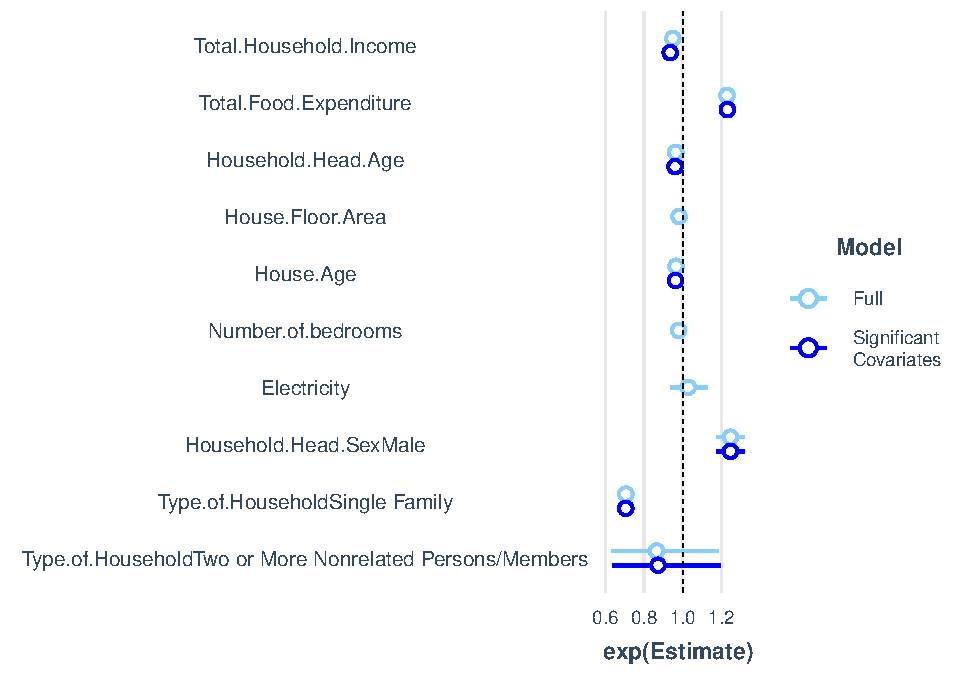
\includegraphics[width=0.8\linewidth]{Group_01_Project2_demo_files/figure-latex/summary plot-1} 

}

\caption{Summary of Coefficients for each fitted Poisson Model}\label{fig:summary plot}
\end{figure}

\begin{figure}[H]

{\centering 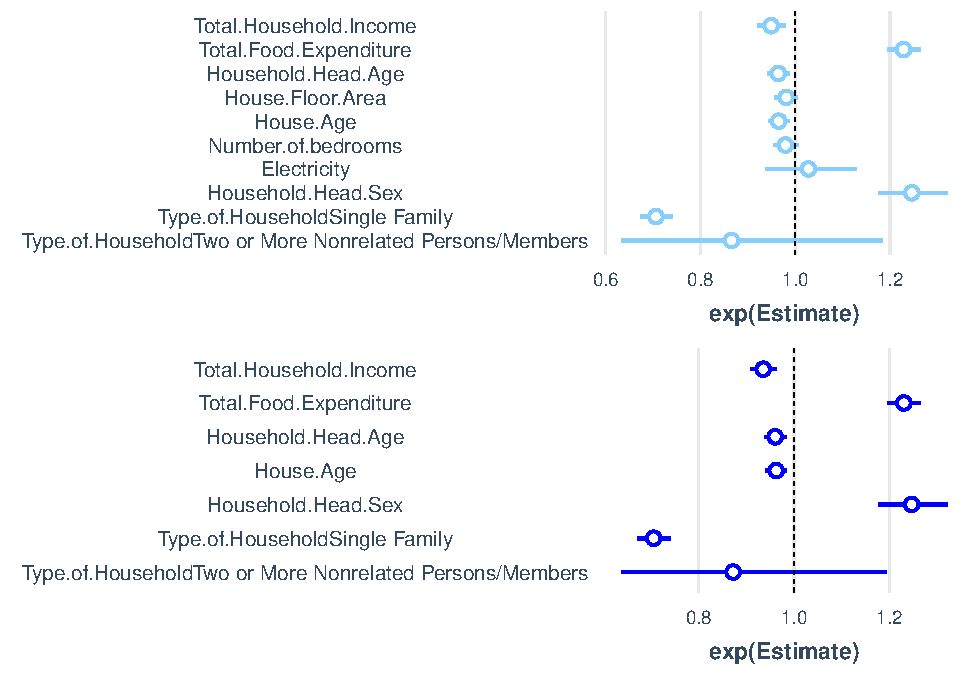
\includegraphics[width=0.8\linewidth]{Group_01_Project2_demo_files/figure-latex/separate summary plots-1} 

}

\caption{Separate summaries of coefficients for the fitted Poisson Models}\label{fig:separate summary plots}
\end{figure}

\begin{longtable}[]{@{}lrr@{}}
\caption{Comparison of Fitted Poisson Models}\tabularnewline
\toprule
Model & AIC & BIC\tabularnewline
\midrule
\endfirsthead
\toprule
Model & AIC & BIC\tabularnewline
\midrule
\endhead
Full Model & 7011.64 & 7071.61\tabularnewline
Significant Factors Model & 7012.00 & 7055.62\tabularnewline
\bottomrule
\end{longtable}

\textless\textless\textless\textless\textless\textless\textless{} HEAD

\begin{figure}[H]

{\centering 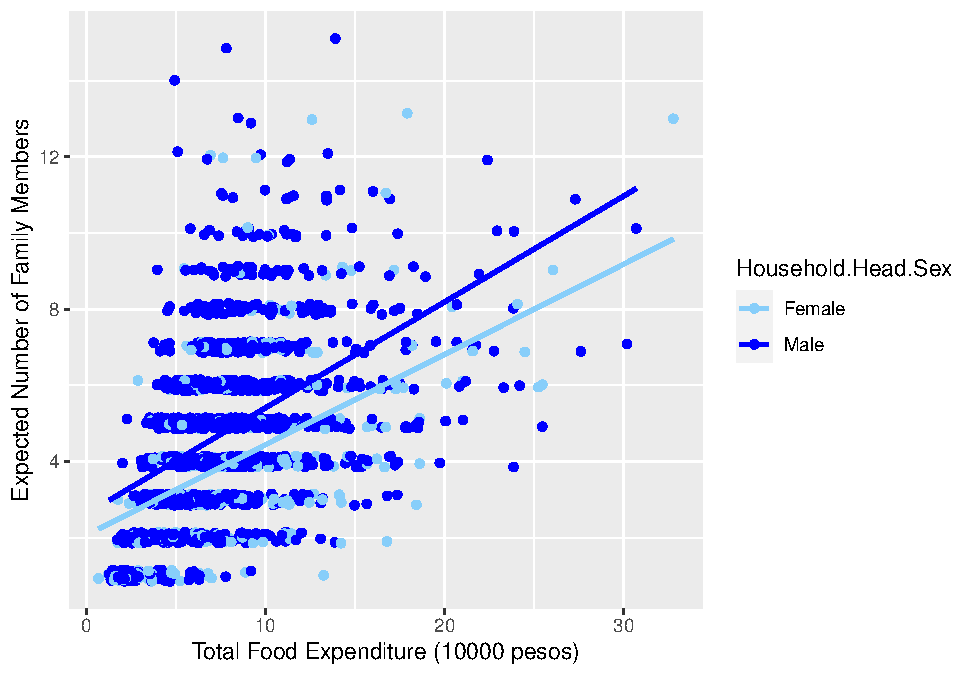
\includegraphics[width=0.8\linewidth]{Group_01_Project2_demo_files/figure-latex/pred plot-1} 

}

\caption{Predicted Numbers of Household Members}\label{fig:pred plot}
\end{figure}

=======

\begin{quote}
\begin{quote}
\begin{quote}
\begin{quote}
\begin{quote}
\begin{quote}
\begin{quote}
0d6ddb30beb8e590d2be4eacc738653ace2af7ea
\end{quote}
\end{quote}
\end{quote}
\end{quote}
\end{quote}
\end{quote}
\end{quote}

\end{document}
